\documentclass{article}

\usepackage{amsmath}
\usepackage{tikz}

\begin{document}

\section{The Rules}

\begin{enumerate}
\item All nodes must be either red or black
\item The root and leaves must be black
\item Red nodes cannot be adjacent
\item All simple paths from a node (exclusive) to a descendent leaf must have the
same number of black nodes
\end{enumerate}

\subsection{Black Height}

Count all black nodes along a simple path from one node to all its descendent
leaves.

\begin{center}
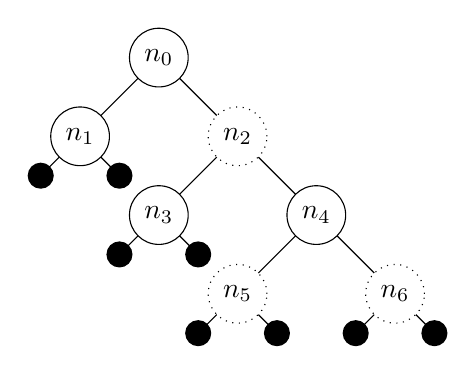
\begin{tikzpicture}
\draw (0,0) -- (-1,-1);
\draw (0,0) -- (1,-1);
\draw (-1,-1) -- (-1.5,-1.5) node[circle,fill=black] {};
\draw (-1,-1) -- (-0.5,-1.5) node[circle,fill=black] {};
\draw (1,-1) -- (0,-2);
\draw (1,-1) -- (2,-2);
\draw (0,-2) -- (-0.5,-2.5) node[circle,fill=black] {};
\draw (0,-2) -- (0.5,-2.5) node[circle,fill=black] {};
\draw (2,-2) -- (1,-3);
\draw (2,-2) -- (3,-3);
\draw (1,-3) -- (0.5,-3.5) node[circle,fill=black] {};
\draw (1,-3) -- (1.5,-3.5) node[circle,fill=black] {};
\draw (3,-3) -- (2.5,-3.5) node[circle,fill=black] {};
\draw (3,-3) -- (3.5,-3.5) node[circle,fill=black] {};

\draw (0,0) node[circle,draw=black,fill=white] {$n_0$};
\draw (-1,-1) node[circle,draw=black,fill=white] {$n_1$};
\draw (1,-1) node[circle,dotted,draw=black,fill=white] {$n_2$};
\draw (0,-2) node[circle,draw=black,fill=white] {$n_3$};
\draw (2,-2) node[circle,draw=black,fill=white] {$n_4$};
\draw (1,-3) node[circle,dotted,draw=black,fill=white] {$n_5$};
\draw (3,-3) node[circle,dotted,draw=black,fill=white] {$n_6$};
\end{tikzpicture}
\end{center}

\begin{equation*}
bh(n_1) = bh(n_3) = bh(n_5) = bh(n_6) = bh(n_4) = 1
\end{equation*}

\begin{equation*}
bh(n_2) = bh(n_0) = 2
\end{equation*}

\subsection{2-3-4 Relationship}

\begin{itemize}
\item All red nodes merge with parents to form a 3 or 4 node.
\item Corresponding 2-3-4 tree has the same height as the black height of the
red-black tree.
\end{itemize}

\section{Insertion}

Keep adding a node strictly less than all other nodes in the tree.  This leads
to imbalance; why?  (I did not specify a color for that node, violating rule
1.)

\subsection{Case 1}

\begin{center}
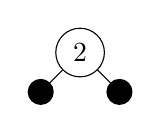
\begin{tikzpicture}
\draw (0,0) -- (-0.5,-0.5) node[circle,fill=black] {};
\draw (0,0) -- (0.5,-0.5) node[circle,fill=black] {};

\draw (0,0) node[circle,draw=black,fill=white] {2};
\end{tikzpicture}
\end{center}

Insert the value 1 into this tree:

\begin{center}
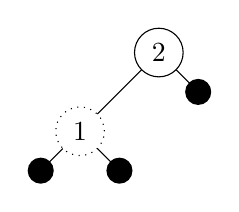
\begin{tikzpicture}
\draw (0,0) -- (-1,-1); 
\draw (0,0) -- (0.5,-0.5) node[circle,fill=black] {};
\draw (-1,-1) -- (-1.5,-1.5) node[circle,fill=black] {};
\draw (-1,-1) -- (-0.5,-1.5) node[circle,fill=black] {};

\draw (0,0) node[circle,draw=black,fill=white] {2};
\draw (-1,-1) node[circle,dotted,draw=black,fill=white] {1};
\end{tikzpicture}
\end{center}

We are done.  This satisfies all properties of a red-black tree!

\subsection{Case 2}

\begin{center}
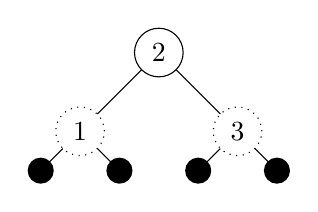
\begin{tikzpicture}
\draw (0,0) -- (-1,-1);
\draw (0,0) -- (1,-1);
\draw (-1,-1) -- (-1.5,-1.5) node[circle,fill=black] {};
\draw (-1,-1) -- (-0.5,-1.5) node[circle,fill=black] {};
\draw (1,-1) -- (0.5,-1.5) node[circle,fill=black] {};
\draw (1,-1) -- (1.5,-1.5) node[circle,fill=black] {};

\draw (0,0) node[circle,draw=black,fill=white] {2};
\draw (-1,-1) node[circle,dotted,draw=black,fill=white] {1};
\draw (1,-1) node[circle,dotted,draw=black,fill=white] {3};
\end{tikzpicture}
\end{center}

Insert a 0 into this tree:

\begin{center}
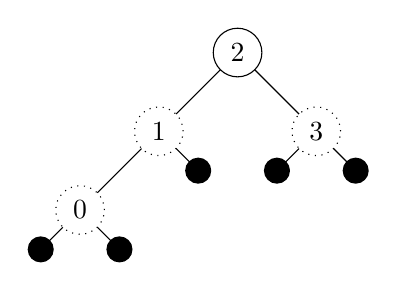
\begin{tikzpicture}
\draw (0,0) -- (-1,-1);
\draw (0,0) -- (1,-1);
\draw (-1,-1) -- (-2,-2);
\draw (-1,-1) -- (-0.5,-1.5) node[circle,fill=black] {};
\draw (1,-1) -- (0.5,-1.5) node[circle,fill=black] {};
\draw (1,-1) -- (1.5,-1.5) node[circle,fill=black] {};
\draw (-2,-2) -- (-2.5,-2.5) node[circle,fill=black] {};
\draw (-2,-2) -- (-1.5,-2.5) node[circle,fill=black] {};

\draw (0,0) node[circle,draw=black,fill=white] {2};
\draw (-1,-1) node[circle,dotted,draw=black,fill=white] {1};
\draw (1,-1) node[circle,dotted,draw=black,fill=white] {3};
\draw (-2,-2) node[circle,dotted,draw=black,fill=white] {0};
\end{tikzpicture}
\end{center}

This violates rule 3, the 0 and 1 nodes are both red, and adjacent.  In this
case, the new node's "uncle" is also red, so we can recolor the graph:

\begin{center}
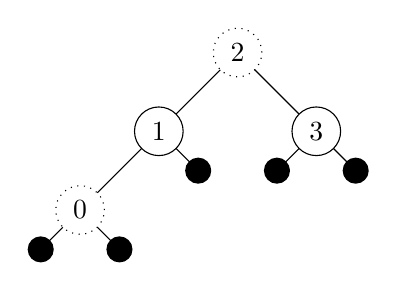
\begin{tikzpicture}
\draw (0,0) -- (-1,-1);
\draw (0,0) -- (1,-1);
\draw (-1,-1) -- (-2,-2);
\draw (-1,-1) -- (-0.5,-1.5) node[circle,fill=black] {};
\draw (1,-1) -- (0.5,-1.5) node[circle,fill=black] {};
\draw (1,-1) -- (1.5,-1.5) node[circle,fill=black] {};
\draw (-2,-2) -- (-2.5,-2.5) node[circle,fill=black] {};
\draw (-2,-2) -- (-1.5,-2.5) node[circle,fill=black] {};

\draw (0,0) node[circle,dotted,draw=black,fill=white] {2};
\draw (-1,-1) node[circle,draw=black,fill=white] {1};
\draw (1,-1) node[circle,draw=black,fill=white] {3};
\draw (-2,-2) node[circle,dotted,draw=black,fill=white] {0};
\end{tikzpicture}
\end{center}

We've now violated a new rule; rule 2.  This is not a big deal though, we can
recolor the root without violating rule 4:

\begin{center}
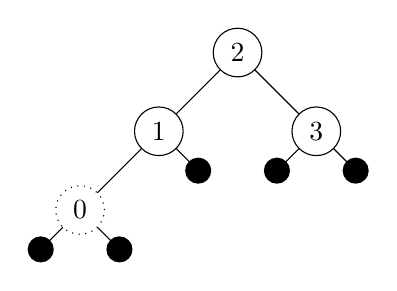
\begin{tikzpicture}
\draw (0,0) -- (-1,-1);
\draw (0,0) -- (1,-1);
\draw (-1,-1) -- (-2,-2);
\draw (-1,-1) -- (-0.5,-1.5) node[circle,fill=black] {};
\draw (1,-1) -- (0.5,-1.5) node[circle,fill=black] {};
\draw (1,-1) -- (1.5,-1.5) node[circle,fill=black] {};
\draw (-2,-2) -- (-2.5,-2.5) node[circle,fill=black] {};
\draw (-2,-2) -- (-1.5,-2.5) node[circle,fill=black] {};

\draw (0,0) node[circle,draw=black,fill=white] {2};
\draw (-1,-1) node[circle,draw=black,fill=white] {1};
\draw (1,-1) node[circle,draw=black,fill=white] {3};
\draw (-2,-2) node[circle,dotted,draw=black,fill=white] {0};
\end{tikzpicture}
\end{center}

In general, you have to work back up the entire tree, starting at the
"grandparent", fixing rule violations as you go.  Here the grandparent was the
root, so we only had to fix one thing.

\subsection{Case 3}

\begin{center}
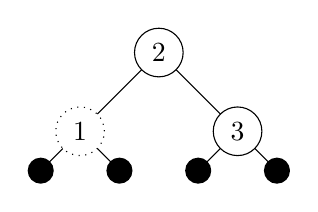
\begin{tikzpicture}
\draw (0,0) -- (-1,-1);
\draw (0,0) -- (1,-1);
\draw (-1,-1) -- (-1.5,-1.5) node[circle,fill=black] {};
\draw (-1,-1) -- (-0.5,-1.5) node[circle,fill=black] {};
\draw (1,-1) -- (0.5,-1.5) node[circle,fill=black] {};
\draw (1,-1) -- (1.5,-1.5) node[circle,fill=black] {};

\draw (0,0) node[circle,draw=black,fill=white] {2};
\draw (-1,-1) node[circle,dotted,draw=black,fill=white] {1};
\draw (1,-1) node[circle,draw=black,fill=white] {3};
\end{tikzpicture}
\end{center}

First off, is this a proper red-black tree?
\begin{itemize}
\item When inserting, we only care about a small portion of the subtree.
\item This, and most future examples, will not themselves be proper red-black trees.
\end{itemize}

Insert 0 into this tree:

\begin{center}
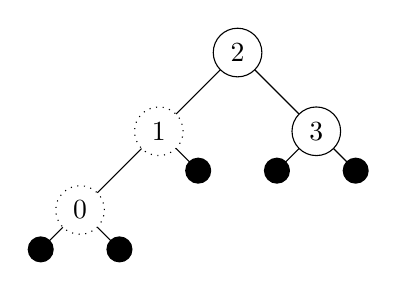
\begin{tikzpicture}
\draw (0,0) -- (-1,-1);
\draw (0,0) -- (1,-1);
\draw (-1,-1) -- (-2,-2);
\draw (-1,-1) -- (-0.5,-1.5) node[circle,fill=black] {};
\draw (1,-1) -- (0.5,-1.5) node[circle,fill=black] {};
\draw (1,-1) -- (1.5,-1.5) node[circle,fill=black] {};
\draw (-2,-2) -- (-2.5,-2.5) node[circle,fill=black] {};
\draw (-2,-2) -- (-1.5,-2.5) node[circle,fill=black] {};

\draw (0,0) node[circle,draw=black,fill=white] {2};
\draw (-1,-1) node[circle,dotted,draw=black,fill=white] {1};
\draw (1,-1) node[circle,draw=black,fill=white] {3};
\draw (-2,-2) node[circle,dotted,draw=black,fill=white] {0};
\end{tikzpicture}
\end{center}

This violates rule 3 again, but the "uncle" node is black, so we cannot
recolor.  We must first rotate:

\begin{center}
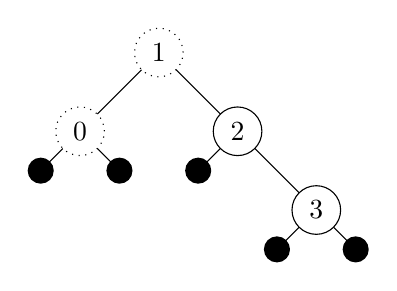
\begin{tikzpicture}
\draw (0,0) -- (-1,-1);
\draw (0,0) -- (1,-1);
\draw (1,-1) -- (2,-2);
\draw (-1,-1) -- (-0.5,-1.5) node[circle,fill=black] {};
\draw (-1,-1) -- (-1.5,-1.5) node[circle,fill=black] {};
\draw (1,-1) -- (0.5,-1.5) node[circle,fill=black] {};
\draw (2,-2) -- (2.5,-2.5) node[circle,fill=black] {};
\draw (2,-2) -- (1.5,-2.5) node[circle,fill=black] {};

\draw (0,0) node[circle,dotted,draw=black,fill=white] {1};
\draw (-1,-1) node[circle,dotted,draw=black,fill=white] {0};
\draw (1,-1) node[circle,draw=black,fill=white] {2};
\draw (2,-2) node[circle,draw=black,fill=white] {3};
\end{tikzpicture}
\end{center}

Then, we may "invert" the color of the rotated nodes (1, 2):

\begin{center}
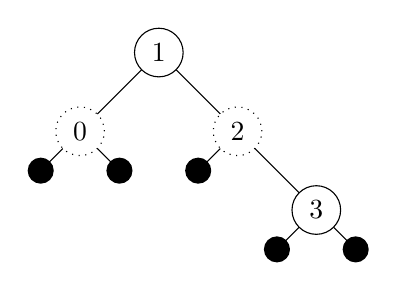
\begin{tikzpicture}
\draw (0,0) -- (-1,-1);
\draw (0,0) -- (1,-1);
\draw (1,-1) -- (2,-2);
\draw (-1,-1) -- (-0.5,-1.5) node[circle,fill=black] {};
\draw (-1,-1) -- (-1.5,-1.5) node[circle,fill=black] {};
\draw (1,-1) -- (0.5,-1.5) node[circle,fill=black] {};
\draw (2,-2) -- (2.5,-2.5) node[circle,fill=black] {};
\draw (2,-2) -- (1.5,-2.5) node[circle,fill=black] {};

\draw (0,0) node[circle,draw=black,fill=white] {1};
\draw (-1,-1) node[circle,dotted,draw=black,fill=white] {0};
\draw (1,-1) node[circle,dotted,draw=black,fill=white] {2};
\draw (2,-2) node[circle,draw=black,fill=white] {3};
\end{tikzpicture}
\end{center}

Here, since we have a black node at our "root", we're done.

\subsection{Case 3, Part 2}

\begin{center}
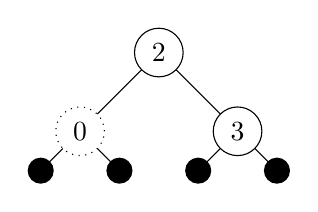
\begin{tikzpicture}
\draw (0,0) -- (-1,-1);
\draw (0,0) -- (1,-1);
\draw (-1,-1) -- (-1.5,-1.5) node[circle,fill=black] {};
\draw (-1,-1) -- (-0.5,-1.5) node[circle,fill=black] {};
\draw (1,-1) -- (0.5,-1.5) node[circle,fill=black] {};
\draw (1,-1) -- (1.5,-1.5) node[circle,fill=black] {};

\draw (0,0) node[circle,draw=black,fill=white] {2};
\draw (-1,-1) node[circle,dotted,draw=black,fill=white] {0};
\draw (1,-1) node[circle,draw=black,fill=white] {3};
\end{tikzpicture}
\end{center}

What if we inserted 1 into this tree?

\begin{center}
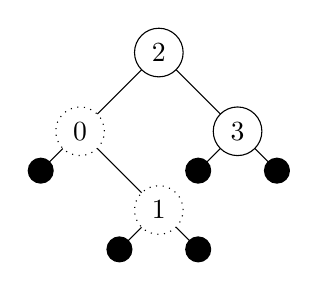
\begin{tikzpicture}
\draw (0,0) -- (-1,-1);
\draw (0,0) -- (1,-1);
\draw (-1,-1) -- (0,-2);
\draw (-1,-1) -- (-1.5,-1.5) node[circle,fill=black] {};
\draw (1,-1) -- (0.5,-1.5) node[circle,fill=black] {};
\draw (1,-1) -- (1.5,-1.5) node[circle,fill=black] {};
\draw (0,-2) -- (-0.5,-2.5) node[circle,fill=black] {};
\draw (0,-2) -- (0.5,-2.5) node[circle,fill=black] {};

\draw (0,0) node[circle,draw=black,fill=white] {2};
\draw (-1,-1) node[circle,dotted,draw=black,fill=white] {0};
\draw (1,-1) node[circle,draw=black,fill=white] {3};
\draw (0,-2) node[circle,dotted,draw=black,fill=white] {1};
\end{tikzpicture}
\end{center}

Looks similar to the previous situation, but we need to do a left-right
rotation before recoloring:

\begin{center}
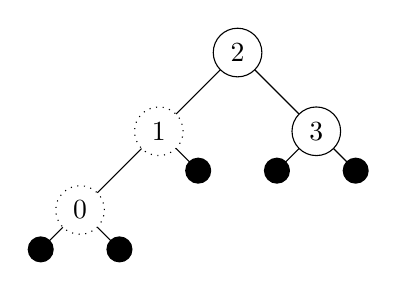
\begin{tikzpicture}
\draw (0,0) -- (-1,-1);
\draw (0,0) -- (1,-1);
\draw (-1,-1) -- (-2,-2);
\draw (-1,-1) -- (-0.5,-1.5) node[circle,fill=black] {};
\draw (1,-1) -- (0.5,-1.5) node[circle,fill=black] {};
\draw (1,-1) -- (1.5,-1.5) node[circle,fill=black] {};
\draw (-2,-2) -- (-2.5,-2.5) node[circle,fill=black] {};
\draw (-2,-2) -- (-1.5,-2.5) node[circle,fill=black] {};

\draw (0,0) node[circle,draw=black,fill=white] {2};
\draw (-1,-1) node[circle,dotted,draw=black,fill=white] {1};
\draw (1,-1) node[circle,draw=black,fill=white] {3};
\draw (-2,-2) node[circle,dotted,draw=black,fill=white] {0};
\end{tikzpicture}
\end{center}

\begin{center}
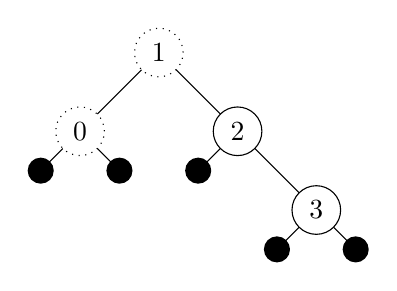
\begin{tikzpicture}
\draw (0,0) -- (-1,-1);
\draw (0,0) -- (1,-1);
\draw (1,-1) -- (2,-2);
\draw (-1,-1) -- (-0.5,-1.5) node[circle,fill=black] {};
\draw (-1,-1) -- (-1.5,-1.5) node[circle,fill=black] {};
\draw (1,-1) -- (0.5,-1.5) node[circle,fill=black] {};
\draw (2,-2) -- (2.5,-2.5) node[circle,fill=black] {};
\draw (2,-2) -- (1.5,-2.5) node[circle,fill=black] {};

\draw (0,0) node[circle,dotted,draw=black,fill=white] {1};
\draw (-1,-1) node[circle,dotted,draw=black,fill=white] {0};
\draw (1,-1) node[circle,draw=black,fill=white] {2};
\draw (2,-2) node[circle,draw=black,fill=white] {3};
\end{tikzpicture}
\end{center}

Then, invert colors as usual:

\begin{center}
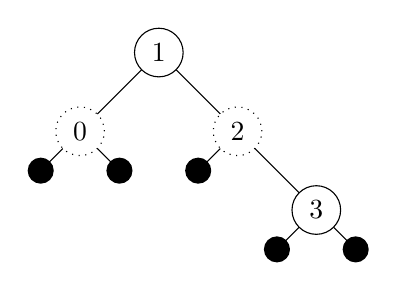
\begin{tikzpicture}
\draw (0,0) -- (-1,-1);
\draw (0,0) -- (1,-1);
\draw (1,-1) -- (2,-2);
\draw (-1,-1) -- (-0.5,-1.5) node[circle,fill=black] {};
\draw (-1,-1) -- (-1.5,-1.5) node[circle,fill=black] {};
\draw (1,-1) -- (0.5,-1.5) node[circle,fill=black] {};
\draw (2,-2) -- (2.5,-2.5) node[circle,fill=black] {};
\draw (2,-2) -- (1.5,-2.5) node[circle,fill=black] {};

\draw (0,0) node[circle,draw=black,fill=white] {1};
\draw (-1,-1) node[circle,dotted,draw=black,fill=white] {0};
\draw (1,-1) node[circle,dotted,draw=black,fill=white] {2};
\draw (2,-2) node[circle,draw=black,fill=white] {3};
\end{tikzpicture}
\end{center}

There are mirrors for right-right, and right-left imbalances.

\section{Putting it All Together}

\begin{center}
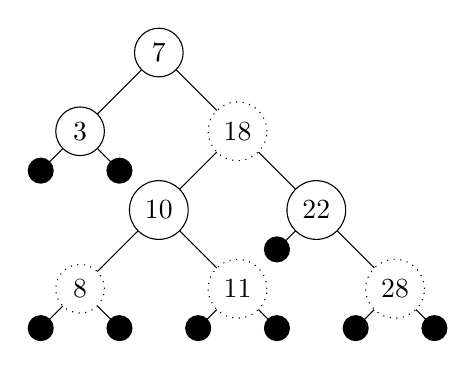
\begin{tikzpicture}
\draw (0,0) -- (-1,-1);
\draw (0,0) -- (1,-1);
\draw (-1,-1) -- (-1.5,-1.5) node[circle,fill=black] {};
\draw (-1,-1) -- (-0.5,-1.5) node[circle,fill=black] {};
\draw (1,-1) -- (0,-2);
\draw (1,-1) -- (2,-2);
\draw (0,-2) -- (-1,-3);
\draw (-1,-3) -- (-1.5,-3.5) node[circle,fill=black] {};
\draw (-1,-3) -- (-0.5,-3.5) node[circle,fill=black] {};
\draw (0,-2) -- (1,-3);
\draw (1,-3) -- (0.5,-3.5) node[circle,fill=black] {};
\draw (1,-3) -- (1.5,-3.5) node[circle,fill=black] {};
\draw (2,-2) -- (1.5,-2.5) node[circle,fill=black] {};
\draw (2,-2) -- (3,-3);
\draw (3,-3) -- (2.5,-3.5) node[circle,fill=black] {};
\draw (3,-3) -- (3.5,-3.5) node[circle,fill=black] {};

\draw (0,0) node[circle,draw=black,fill=white] {7};
\draw (-1,-1) node[circle,draw=black,fill=white] {3};
\draw (1,-1) node[circle,dotted,draw=black,fill=white] {18};
\draw (0,-2) node[circle,draw=black,fill=white] {10};
\draw (2,-2) node[circle,draw=black,fill=white] {22};
\draw (-1,-3) node[circle,dotted,draw=black,fill=white] {8};
\draw (1,-3) node[circle,dotted,draw=black,fill=white] {11};
\draw (3,-3) node[circle,dotted,draw=black,fill=white] {28};
\end{tikzpicture}
\end{center}

Insert 15 into this tree.

\section{Deletion}

\subsection{Case 1}

If you are deleting a red node with a black child, simply move that child up
into the deleted node's place.

\begin{center}
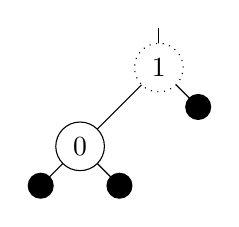
\begin{tikzpicture}
\draw (0,0.5) -- (0,0);
\draw (0,0) -- (0.5,-0.5) node[circle,fill=black] {};
\draw (0,0) -- (-1,-1);
\draw (-1,-1) -- (-1.5,-1.5) node[circle,fill=black] {};
\draw (-1,-1) -- (-0.5,-1.5) node[circle,fill=black] {};

\draw (0,0) node[circle,dotted,draw=black,fill=white] {1};
\draw (-1,-1) node[circle,draw=black,fill=white] {0};
\end{tikzpicture}
\end{center}

\begin{center}
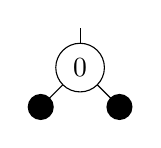
\begin{tikzpicture}
\draw (0,0.5) -- (0,0);
\draw (0,0) -- (-0.5,-0.5) node[circle,fill=black] {};
\draw (0,0) -- (0.5,-0.5) node[circle,fill=black] {};

\draw (0,0) node[circle,draw=black,fill=white] {0};
\end{tikzpicture}
\end{center}

\subsection{Case 2}

If you are deleting a black node with a red child, simply move that child up,
and recolor:

\begin{center}
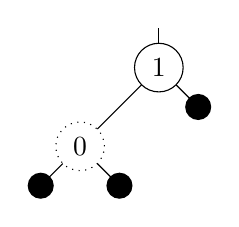
\begin{tikzpicture}
\draw (0,0.5) -- (0,0);
\draw (0,0) -- (0.5,-0.5) node[circle,fill=black] {};
\draw (0,0) -- (-1,-1);
\draw (-1,-1) -- (-1.5,-1.5) node[circle,fill=black] {};
\draw (-1,-1) -- (-0.5,-1.5) node[circle,fill=black] {};

\draw (0,0) node[circle,draw=black,fill=white] {1};
\draw (-1,-1) node[circle,dotted,draw=black,fill=white] {0};
\end{tikzpicture}
\end{center}

\begin{center}
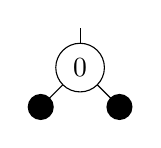
\begin{tikzpicture}
\draw (0,0.5) -- (0,0);
\draw (0,0) -- (-0.5,-0.5) node[circle,fill=black] {};
\draw (0,0) -- (0.5,-0.5) node[circle,fill=black] {};

\draw (0,0) node[circle,draw=black,fill=white] {0};
\end{tikzpicture}
\end{center}

\subsection{Case 3}

If they are both black, there is a potential problem.  We have to introduce a
``double-black'' node to keep track of where this problem exists.

\begin{center}
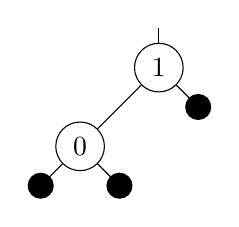
\begin{tikzpicture}
\draw (0,0.5) -- (0,0);
\draw (0,0) -- (0.5,-0.5) node[circle,fill=black] {};
\draw (0,0) -- (-1,-1);
\draw (-1,-1) -- (-1.5,-1.5) node[circle,fill=black] {};
\draw (-1,-1) -- (-0.5,-1.5) node[circle,fill=black] {};

\draw (0,0) node[circle,draw=black,fill=white] {1};
\draw (-1,-1) node[circle,draw=black,fill=white] {0};
\end{tikzpicture}
\end{center}

\begin{center}
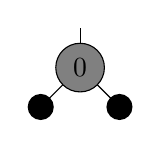
\begin{tikzpicture}
\draw (0,0.5) -- (0,0);
\draw (0,0) -- (-0.5,-0.5) node[circle,fill=black] {};
\draw (0,0) -- (0.5,-0.5) node[circle,fill=black] {};

\draw (0,0) node[circle,draw=black,fill=gray] {0};
\end{tikzpicture}
\end{center}

\subsubsection{Case 3a (Terminal)}

If the node to be deleted was the root, we're fine.  The black height just
reduces by one.

\begin{center}
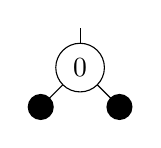
\begin{tikzpicture}
\draw (0,0.5) -- (0,0);
\draw (0,0) -- (-0.5,-0.5) node[circle,fill=black] {};
\draw (0,0) -- (0.5,-0.5) node[circle,fill=black] {};

\draw (0,0) node[circle,draw=black,fill=white] {0};
\end{tikzpicture}
\end{center}

\subsubsection{Case 3b}

If there is a sibling node that is red, we have to rotate to eliminate the
double-black node:

\begin{center}
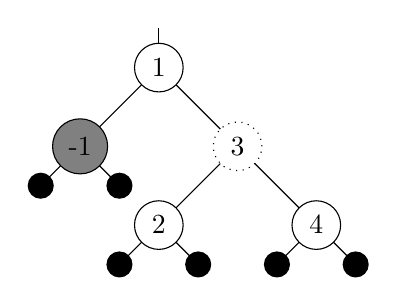
\begin{tikzpicture}
\draw (0,0.5) -- (0,0);
\draw (0,0) -- (-1,-1);
\draw (0,0) -- (1,-1);
\draw (1,-1) -- (0,-2);
\draw (1,-1) -- (2,-2);
\draw (-1,-1) -- (-1.5,-1.5) node[circle,fill=black] {};
\draw (-1,-1) -- (-0.5,-1.5) node[circle,fill=black] {};
\draw (0,-2) -- (-0.5,-2.5) node[circle,fill=black] {};
\draw (0,-2) -- (0.5,-2.5) node[circle,fill=black] {};
\draw (2,-2) -- (1.5,-2.5) node[circle,fill=black] {};
\draw (2,-2) -- (2.5,-2.5) node[circle,fill=black] {};

\draw (0,0) node[circle,draw=black,fill=white] {1};
\draw (-1,-1) node[circle,draw=black,fill=gray] {-1};
\draw (1,-1) node[circle,dotted,draw=black,fill=white] {3};
\draw (0,-2) node[circle,draw=black,fill=white] {2};
\draw (2,-2) node[circle,draw=black,fill=white] {4};
\end{tikzpicture}
\end{center}

\begin{center}
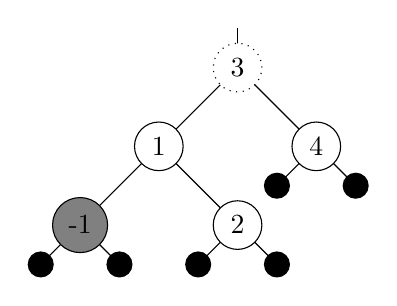
\begin{tikzpicture}
\draw (0,0.5) -- (0,0);
\draw (0,0) -- (-1,-1);
\draw (0,0) -- (1,-1);
\draw (1,-1) -- (0.5,-1.5) node[circle,fill=black] {};
\draw (1,-1) -- (1.5,-1.5) node[circle,fill=black] {};
\draw (-1,-1) -- (0,-2);
\draw (-1,-1) -- (-2,-2);
\draw (0,-2) -- (-0.5,-2.5) node[circle,fill=black] {};
\draw (0,-2) -- (0.5,-2.5) node[circle,fill=black] {};
\draw (-2,-2) -- (-2.5,-2.5) node[circle,fill=black] {};
\draw (-2,-2) -- (-1.5,-2.5) node[circle,fill=black] {};

\draw (0,0) node[circle,dotted,draw=black,fill=white] {3};
\draw (-1,-1) node[circle,draw=black,fill=white] {1};
\draw (1,-1) node[circle,draw=black,fill=white] {4};
\draw (0,-2) node[circle,draw=black,fill=white] {2};
\draw (-2,-2) node[circle,draw=black,fill=gray] {-1};
\end{tikzpicture}
\end{center}

Then, we have to recolor the 1 and 3 nodes.

\begin{center}
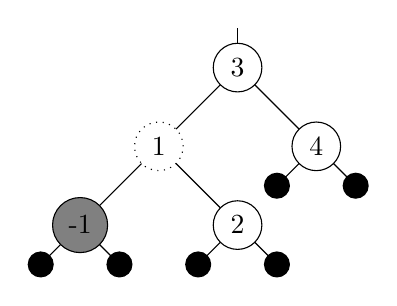
\begin{tikzpicture}
\draw (0,0.5) -- (0,0);
\draw (0,0) -- (-1,-1);
\draw (0,0) -- (1,-1);
\draw (1,-1) -- (0.5,-1.5) node[circle,fill=black] {};
\draw (1,-1) -- (1.5,-1.5) node[circle,fill=black] {};
\draw (-1,-1) -- (0,-2);
\draw (-1,-1) -- (-2,-2);
\draw (0,-2) -- (-0.5,-2.5) node[circle,fill=black] {};
\draw (0,-2) -- (0.5,-2.5) node[circle,fill=black] {};
\draw (-2,-2) -- (-2.5,-2.5) node[circle,fill=black] {};
\draw (-2,-2) -- (-1.5,-2.5) node[circle,fill=black] {};

\draw (0,0) node[circle,draw=black,fill=white] {3};
\draw (-1,-1) node[circle,dotted,draw=black,fill=white] {1};
\draw (1,-1) node[circle,draw=black,fill=white] {4};
\draw (0,-2) node[circle,draw=black,fill=white] {2};
\draw (-2,-2) node[circle,draw=black,fill=gray] {-1};
\end{tikzpicture}
\end{center}

We have to now continue to a new case.

\subsubsection{Case 3c}

If the sibling node is black, and both of its children are black, recolor the
sibling and move up

\begin{center}
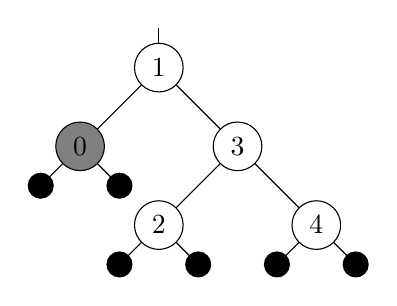
\begin{tikzpicture}
\draw (0,0.5) -- (0,0);
\draw (0,0) -- (-1,-1);
\draw (0,0) -- (1,-1);
\draw (1,-1) -- (0,-2);
\draw (1,-1) -- (2,-2);
\draw (0,-2) -- (-0.5,-2.5) node[circle,fill=black] {};
\draw (0,-2) -- (0.5,-2.5) node[circle,fill=black] {};
\draw (-1,-1) -- (-1.5,-1.5) node[circle,fill=black] {};
\draw (-1,-1) -- (-0.5,-1.5) node[circle,fill=black] {};
\draw (2,-2) -- (1.5,-2.5) node[circle,fill=black] {};
\draw (2,-2) -- (2.5,-2.5) node[circle,fill=black] {};

\draw (0,0) node[circle,draw=black,fill=white] {1};
\draw (-1,-1) node[circle,draw=black,fill=gray] {0};
\draw (1,-1) node[circle,draw=black,fill=white] {3};
\draw (0,-2) node[circle,draw=black,fill=white] {2};
\draw (2,-2) node[circle,draw=black,fill=white] {4};
\end{tikzpicture}
\end{center}

\begin{center}
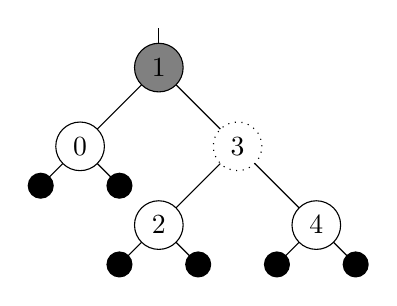
\begin{tikzpicture}
\draw (0,0.5) -- (0,0);
\draw (0,0) -- (-1,-1);
\draw (0,0) -- (1,-1);
\draw (1,-1) -- (0,-2);
\draw (1,-1) -- (2,-2);
\draw (0,-2) -- (-0.5,-2.5) node[circle,fill=black] {};
\draw (0,-2) -- (0.5,-2.5) node[circle,fill=black] {};
\draw (-1,-1) -- (-1.5,-1.5) node[circle,fill=black] {};
\draw (-1,-1) -- (-0.5,-1.5) node[circle,fill=black] {};
\draw (2,-2) -- (1.5,-2.5) node[circle,fill=black] {};
\draw (2,-2) -- (2.5,-2.5) node[circle,fill=black] {};

\draw (0,0) node[circle,draw=black,fill=gray] {1};
\draw (-1,-1) node[circle,draw=black,fill=white] {0};
\draw (1,-1) node[circle,dotted,draw=black,fill=white] {3};
\draw (0,-2) node[circle,draw=black,fill=white] {2};
\draw (2,-2) node[circle,draw=black,fill=white] {4};
\end{tikzpicture}
\end{center}

\subsubsection{Case 3d (Terminal)}

If the sibling is black, and the parent is red:

\begin{center}
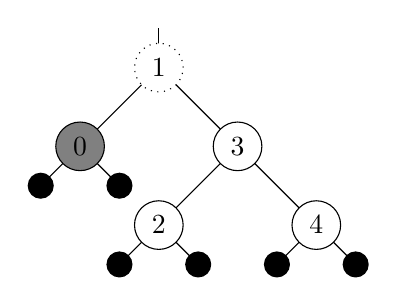
\begin{tikzpicture}
\draw (0,0.5) -- (0,0);
\draw (0,0) -- (-1,-1);
\draw (0,0) -- (1,-1);
\draw (1,-1) -- (0,-2);
\draw (1,-1) -- (2,-2);
\draw (0,-2) -- (-0.5,-2.5) node[circle,fill=black] {};
\draw (0,-2) -- (0.5,-2.5) node[circle,fill=black] {};
\draw (-1,-1) -- (-1.5,-1.5) node[circle,fill=black] {};
\draw (-1,-1) -- (-0.5,-1.5) node[circle,fill=black] {};
\draw (2,-2) -- (1.5,-2.5) node[circle,fill=black] {};
\draw (2,-2) -- (2.5,-2.5) node[circle,fill=black] {};

\draw (0,0) node[circle,dotted,draw=black,fill=white] {1};
\draw (-1,-1) node[circle,draw=black,fill=gray] {0};
\draw (1,-1) node[circle,draw=black,fill=white] {3};
\draw (0,-2) node[circle,draw=black,fill=white] {2};
\draw (2,-2) node[circle,draw=black,fill=white] {4};
\end{tikzpicture}
\end{center}

Recolor, and you're done:

\begin{center}
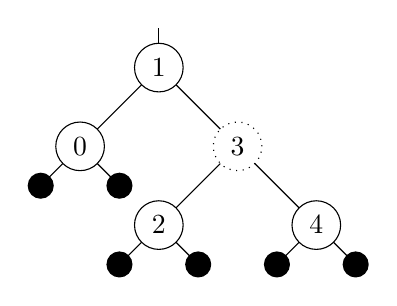
\begin{tikzpicture}
\draw (0,0.5) -- (0,0);
\draw (0,0) -- (-1,-1);
\draw (0,0) -- (1,-1);
\draw (1,-1) -- (0,-2);
\draw (1,-1) -- (2,-2);
\draw (0,-2) -- (-0.5,-2.5) node[circle,fill=black] {};
\draw (0,-2) -- (0.5,-2.5) node[circle,fill=black] {};
\draw (-1,-1) -- (-1.5,-1.5) node[circle,fill=black] {};
\draw (-1,-1) -- (-0.5,-1.5) node[circle,fill=black] {};
\draw (2,-2) -- (1.5,-2.5) node[circle,fill=black] {};
\draw (2,-2) -- (2.5,-2.5) node[circle,fill=black] {};

\draw (0,0) node[circle,draw=black,fill=white] {1};
\draw (-1,-1) node[circle,draw=black,fill=white] {0};
\draw (1,-1) node[circle,dotted,draw=black,fill=white] {3};
\draw (0,-2) node[circle,draw=black,fill=white] {2};
\draw (2,-2) node[circle,draw=black,fill=white] {4};
\end{tikzpicture}
\end{center}

\subsubsection{Case 3e}

If the parent, sibling, and sibling's right child are black, but the sibling's
left child is red:

\begin{center}
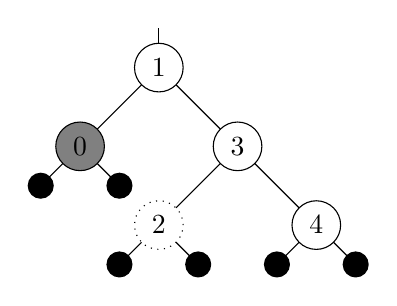
\begin{tikzpicture}
\draw (0,0.5) -- (0,0);
\draw (0,0) -- (-1,-1);
\draw (0,0) -- (1,-1);
\draw (1,-1) -- (0,-2);
\draw (1,-1) -- (2,-2);
\draw (0,-2) -- (-0.5,-2.5) node[circle,fill=black] {};
\draw (0,-2) -- (0.5,-2.5) node[circle,fill=black] {};
\draw (-1,-1) -- (-1.5,-1.5) node[circle,fill=black] {};
\draw (-1,-1) -- (-0.5,-1.5) node[circle,fill=black] {};
\draw (2,-2) -- (1.5,-2.5) node[circle,fill=black] {};
\draw (2,-2) -- (2.5,-2.5) node[circle,fill=black] {};

\draw (0,0) node[circle,draw=black,fill=white] {1};
\draw (-1,-1) node[circle,draw=black,fill=gray] {0};
\draw (1,-1) node[circle,draw=black,fill=white] {3};
\draw (0,-2) node[circle,dotted,draw=black,fill=white] {2};
\draw (2,-2) node[circle,draw=black,fill=white] {4};
\end{tikzpicture}
\end{center}

You must rotate to make the sibling's right child red:

\begin{center}
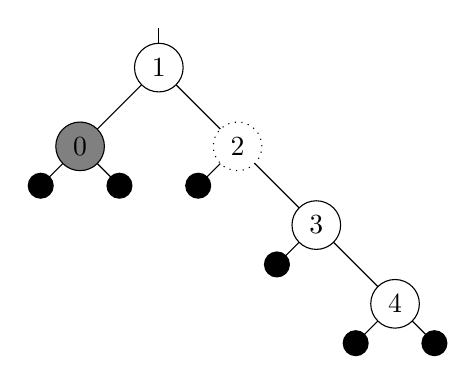
\begin{tikzpicture}
\draw (0,0.5) -- (0,0);
\draw (0,0) -- (-1,-1);
\draw (0,0) -- (1,-1);
\draw (1,-1) -- (0.5,-1.5) node[circle,fill=black] {};
\draw (1,-1) -- (2,-2);
\draw (2,-2) -- (3,-3);
\draw (-1,-1) -- (-1.5,-1.5) node[circle,fill=black] {};
\draw (-1,-1) -- (-0.5,-1.5) node[circle,fill=black] {};
\draw (2,-2) -- (1.5,-2.5) node[circle,fill=black] {};
\draw (3,-3) -- (2.5,-3.5) node[circle,fill=black] {};
\draw (3,-3) -- (3.5,-3.5) node[circle,fill=black] {};

\draw (0,0) node[circle,draw=black,fill=white] {1};
\draw (-1,-1) node[circle,draw=black,fill=gray] {0};
\draw (1,-1) node[circle,dotted,draw=black,fill=white] {2};
\draw (2,-2) node[circle,draw=black,fill=white] {3};
\draw (3,-3) node[circle,draw=black,fill=white] {4};
\end{tikzpicture}
\end{center}

Don't forget to recolor:

\begin{center}
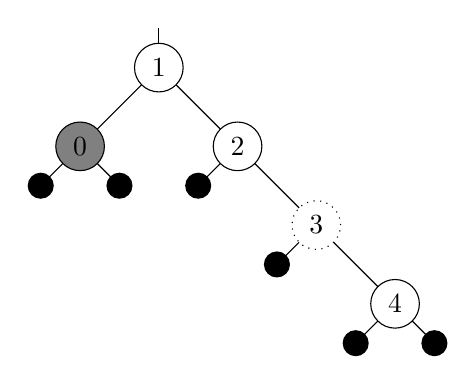
\begin{tikzpicture}
\draw (0,0.5) -- (0,0);
\draw (0,0) -- (-1,-1);
\draw (0,0) -- (1,-1);
\draw (1,-1) -- (0.5,-1.5) node[circle,fill=black] {};
\draw (1,-1) -- (2,-2);
\draw (2,-2) -- (3,-3);
\draw (-1,-1) -- (-1.5,-1.5) node[circle,fill=black] {};
\draw (-1,-1) -- (-0.5,-1.5) node[circle,fill=black] {};
\draw (2,-2) -- (1.5,-2.5) node[circle,fill=black] {};
\draw (3,-3) -- (2.5,-3.5) node[circle,fill=black] {};
\draw (3,-3) -- (3.5,-3.5) node[circle,fill=black] {};

\draw (0,0) node[circle,draw=black,fill=white] {1};
\draw (-1,-1) node[circle,draw=black,fill=gray] {0};
\draw (1,-1) node[circle,draw=black,fill=white] {2};
\draw (2,-2) node[circle,dotted,draw=black,fill=white] {3};
\draw (3,-3) node[circle,draw=black,fill=white] {4};
\end{tikzpicture}
\end{center}

Then, continue on to the next case.

\subsubsection{Case 3f (Terminal)}

If the parent and sibling are black, but the sibling's right child is red:

\begin{center}
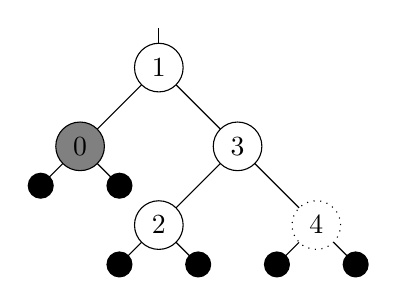
\begin{tikzpicture}
\draw (0,0.5) -- (0,0);
\draw (0,0) -- (-1,-1);
\draw (0,0) -- (1,-1);
\draw (1,-1) -- (0,-2);
\draw (1,-1) -- (2,-2);
\draw (0,-2) -- (-0.5,-2.5) node[circle,fill=black] {};
\draw (0,-2) -- (0.5,-2.5) node[circle,fill=black] {};
\draw (-1,-1) -- (-1.5,-1.5) node[circle,fill=black] {};
\draw (-1,-1) -- (-0.5,-1.5) node[circle,fill=black] {};
\draw (2,-2) -- (1.5,-2.5) node[circle,fill=black] {};
\draw (2,-2) -- (2.5,-2.5) node[circle,fill=black] {};

\draw (0,0) node[circle,draw=black,fill=white] {1};
\draw (-1,-1) node[circle,draw=black,fill=gray] {0};
\draw (1,-1) node[circle,draw=black,fill=white] {3};
\draw (0,-2) node[circle,draw=black,fill=white] {2};
\draw (2,-2) node[circle,dotted,draw=black,fill=white] {4};
\end{tikzpicture}
\end{center}

You must rotate (to the left) around the parent:

\begin{center}
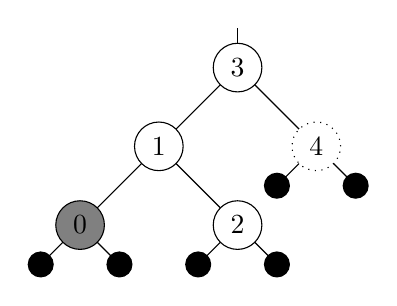
\begin{tikzpicture}
\draw (0,0.5) -- (0,0);
\draw (0,0) -- (-1,-1);
\draw (0,0) -- (1,-1);
\draw (-1,-1) -- (0,-2);
\draw (-1,-1) -- (-2,-2);
\draw (-2,-2) -- (-1.5,-2.5) node[circle,fill=black] {};
\draw (-2,-2) -- (-2.5,-2.5) node[circle,fill=black] {};
\draw (0,-2) -- (-0.5,-2.5) node[circle,fill=black] {};
\draw (0,-2) -- (0.5,-2.5) node[circle,fill=black] {};
\draw (1,-1) -- (0.5,-1.5) node[circle,fill=black] {};
\draw (1,-1) -- (1.5,-1.5) node[circle,fill=black] {};

\draw (0,0) node[circle,draw=black,fill=white] {3};
\draw (-1,-1) node[circle,draw=black,fill=white] {1};
\draw (1,-1) node[circle,dotted,draw=black,fill=white] {4};
\draw (0,-2) node[circle,draw=black,fill=white] {2};
\draw (-2,-2) node[circle,draw=black,fill=gray] {0};
\end{tikzpicture}
\end{center}

Recolor, and you're done:

\begin{center}
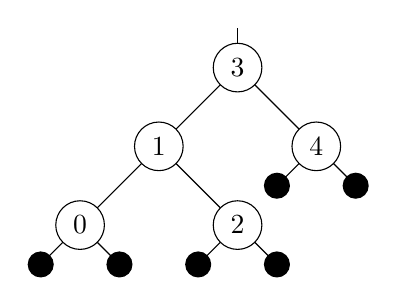
\begin{tikzpicture}
\draw (0,0.5) -- (0,0);
\draw (0,0) -- (-1,-1);
\draw (0,0) -- (1,-1);
\draw (-1,-1) -- (0,-2);
\draw (-1,-1) -- (-2,-2);
\draw (-2,-2) -- (-1.5,-2.5) node[circle,fill=black] {};
\draw (-2,-2) -- (-2.5,-2.5) node[circle,fill=black] {};
\draw (0,-2) -- (-0.5,-2.5) node[circle,fill=black] {};
\draw (0,-2) -- (0.5,-2.5) node[circle,fill=black] {};
\draw (1,-1) -- (0.5,-1.5) node[circle,fill=black] {};
\draw (1,-1) -- (1.5,-1.5) node[circle,fill=black] {};

\draw (0,0) node[circle,draw=black,fill=white] {3};
\draw (-1,-1) node[circle,draw=black,fill=white] {1};
\draw (1,-1) node[circle,draw=black,fill=white] {4};
\draw (0,-2) node[circle,draw=black,fill=white] {2};
\draw (-2,-2) node[circle,draw=black,fill=white] {0};
\end{tikzpicture}
\end{center}

\end{document}
